There are\footnote{This section is stolen from Ref.~\cite{Ilten:2017rbd} and has benefited from conversations with Peter Skands.} several aspects of the $g\rightarrow b\bar{b}$ decay that would provide nearly direct measurements of the fragmentation function.  Three key variables are\footnote{Plots for the unnormalized mass can be found in Appendix~\ref{sec:app-trkmass}.} $\Delta R(b,\bar{b}), \rho_{b\bar{b}}=m_{b\bar{b}}/p_\text{T,$b\bar{b}$}$, and $z_{b\bar{b}}=p_\text{b}/p_\text{T,g}$.  None of the distributions of these quantities have been measured for $\Delta R(b,\bar{b}) < R$ ($R=$ jet radius).  Figure~\ref{fig:gbb-gbbdistributions} shows the distribution of these three variables, as predicted by Pythia~\cite{Pythia8}.  In addition to the nominal prediction, the sensitivity to variations in the modeling of fragmentation is illustrated by varying parameters in Pythia~\cite{pythiavariations}.  The variables sensitive to the $b\bar{b}$ opening angle ($\Delta R$ and mass) have 10\% variations due to the scale variations in the fragmentation.  There are likely other variations that these observables are sensitive to, such as the quark mass effects.

One of the key choices in this measurement is deciding to unfold to less observable quantities ($b$-quarks), more observable quantities ($b$-jets or $b$ track-jets), or somewhere in between ($B$-hadrons).  The impact of this choice is illustrated in Fig.~\ref{fig:gbb-gbbresponse}.  For $\Delta R$, all choices give similar answers.  Unsurprisingly, the momentum fraction is more sensitive to the choice of unfolding target.  In order to have access to small angular scales without needing to explicitly reconstruct $B$-hadrons, we use small-radius track jets.

In addition to the QCD properties of the fragmentation, one can also make measurements of observables that are sensitive to the gluon spin, as in the angle between the gluon production and gluon `decay' planes shown in Fig.~\ref{fig:gbb-gbbangle}.

\begin{figure}[htpb!]
\begin{center}
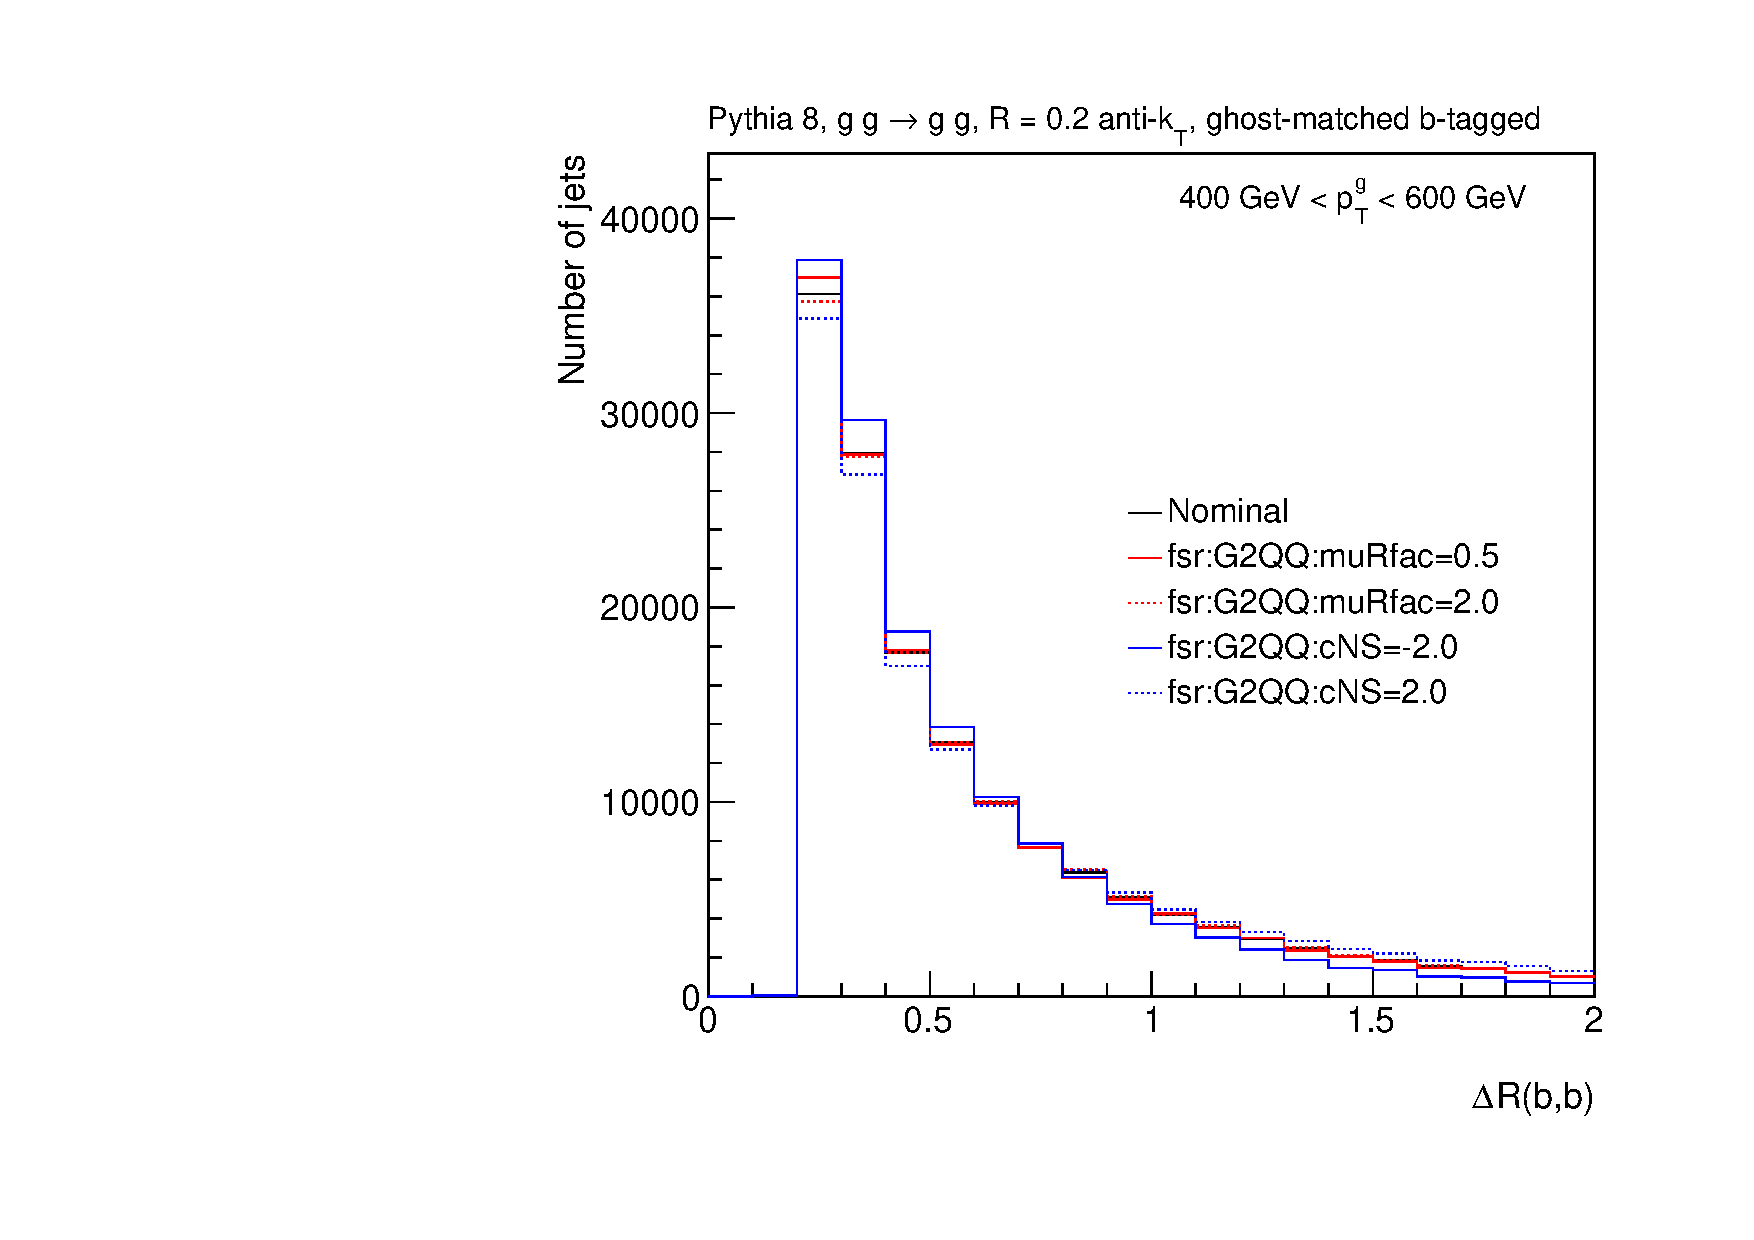
\includegraphics[width=0.33\linewidth]{figures/gbb/truth_level/DeltaRbb.pdf}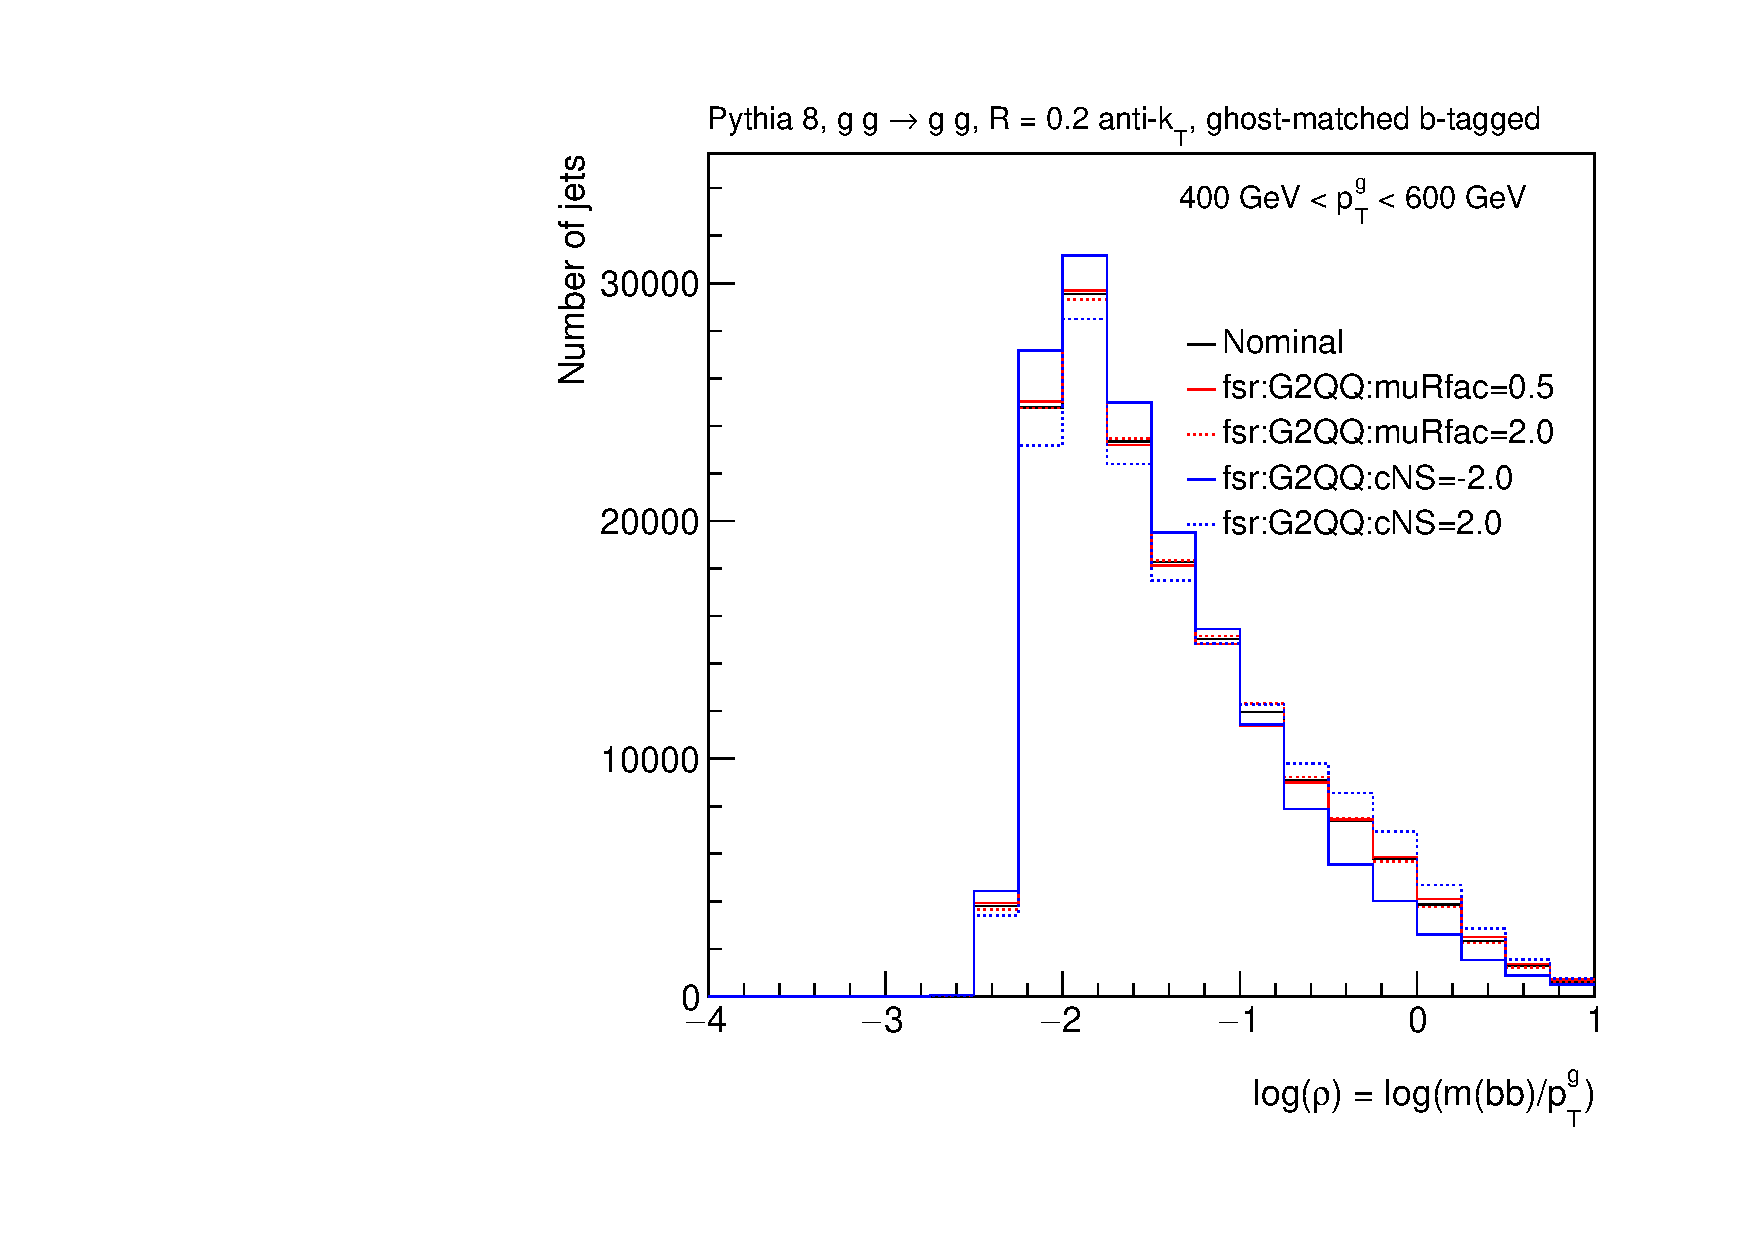
\includegraphics[width=0.33\linewidth]{figures/gbb/truth_level/rhobb.pdf}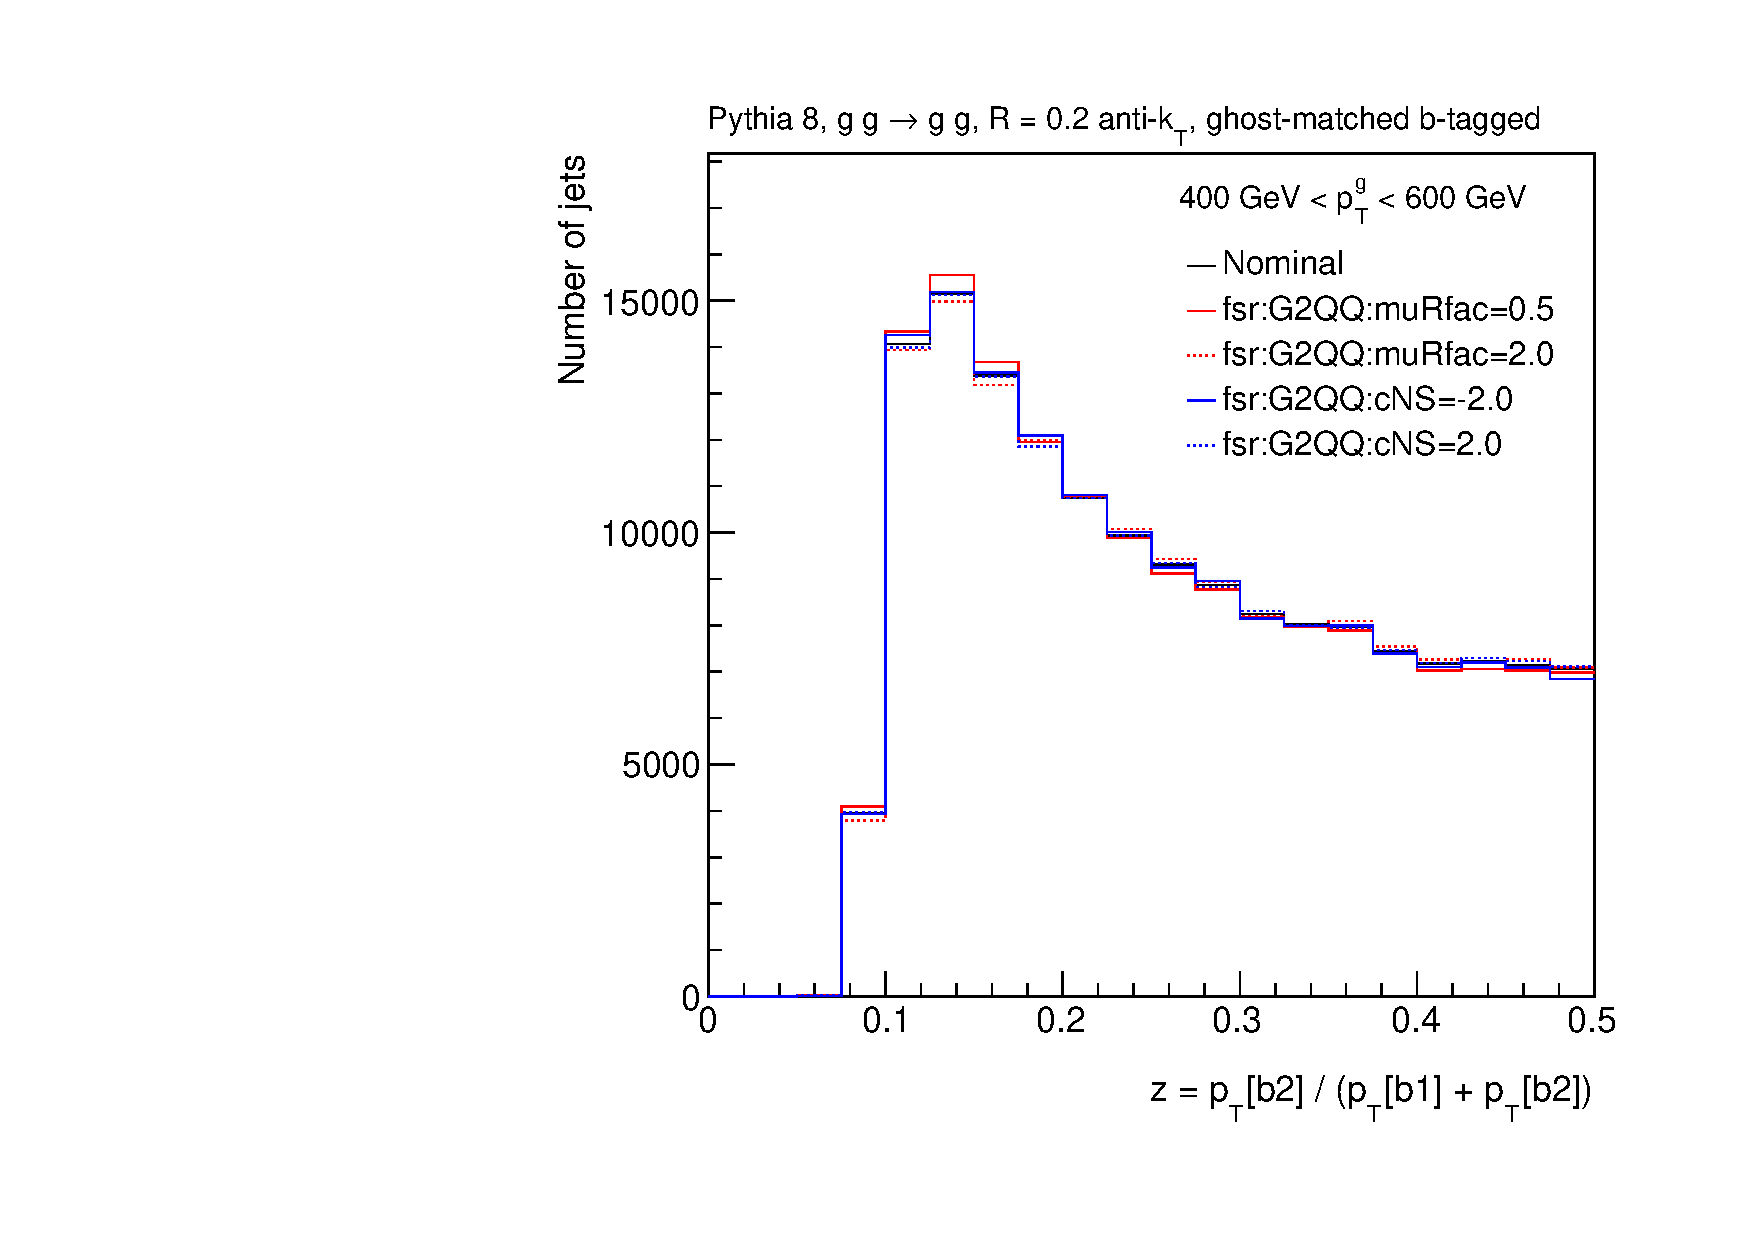
\includegraphics[width=0.33\linewidth]{figures/gbb/truth_level/DeltaZbb.pdf}
\caption{The distributions of $\Delta R(b,\bar{b}), \rho_{b\bar{b}}=m_{b\bar{b}}/p_\text{T,$b\bar{b}$}$, and $z_{b\bar{b}}=p_\text{b}/p_\text{T,g}$ in simulation along with a series of variations in the form of the fragmentation described by Pythia~\cite{pythiavariations}.} 
\label{fig:gbb-gbbdistributions}
\end{center}
\end{figure}

\begin{figure}[htpb!]
\begin{center}
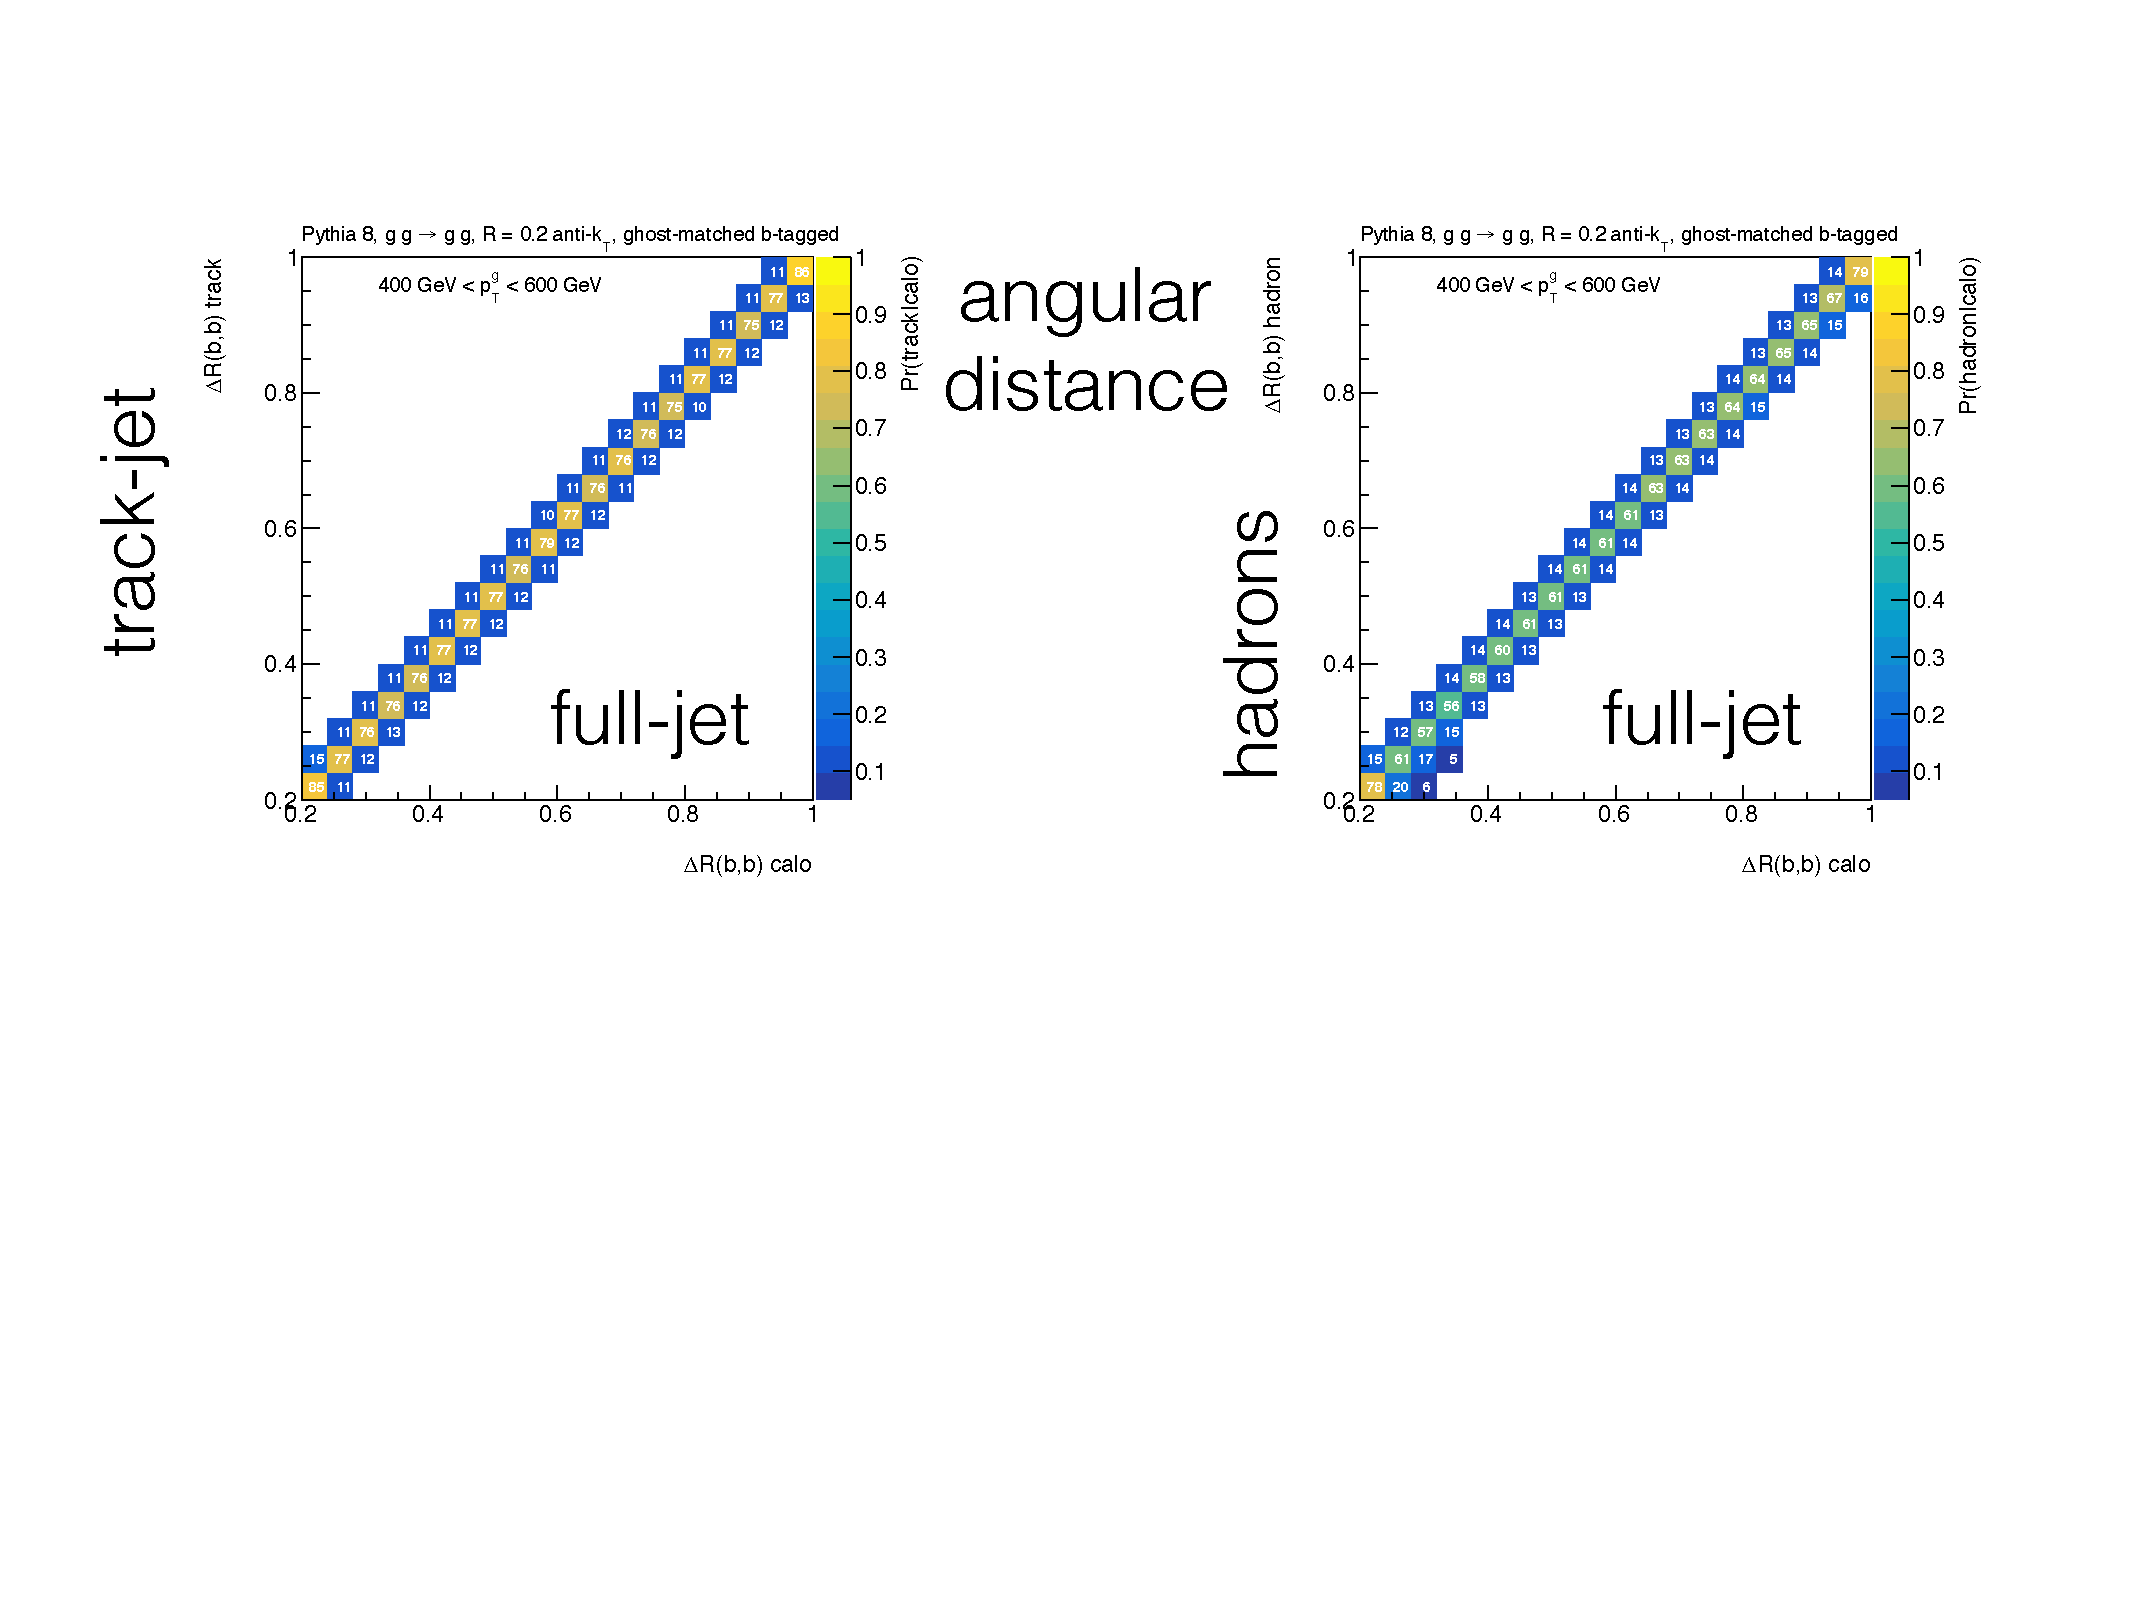
\includegraphics[width=0.95\linewidth]{figures/gbb/truth_level/compare2.pdf}\\
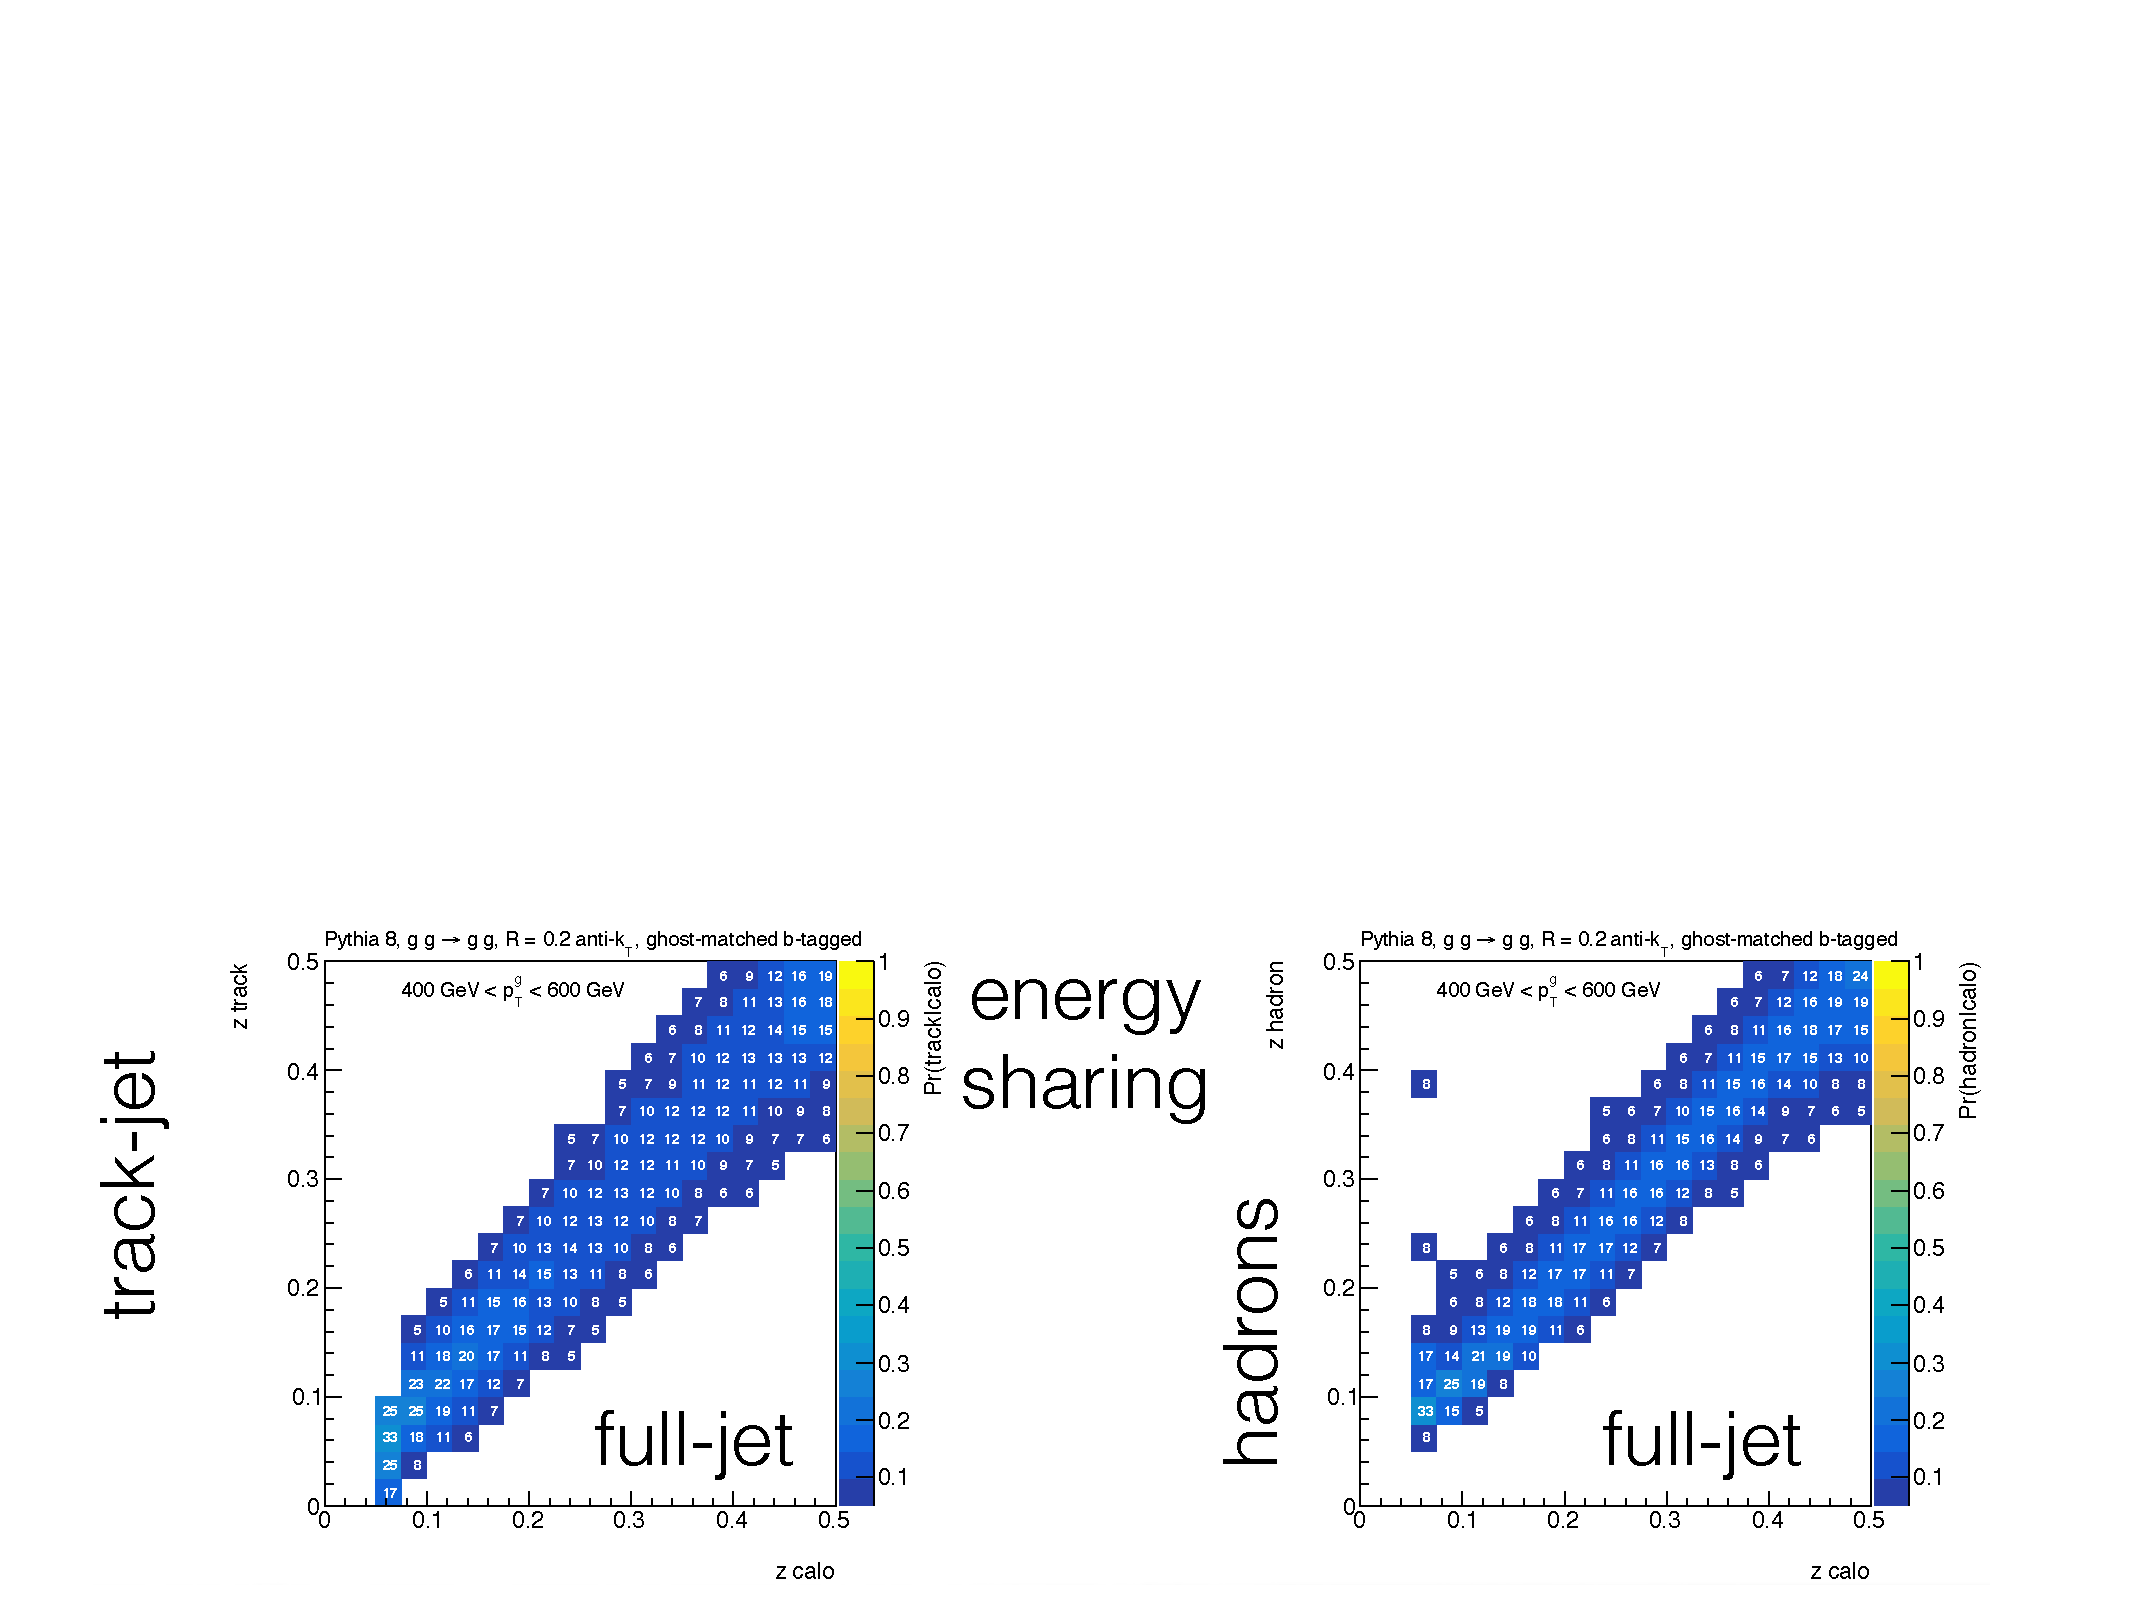
\includegraphics[width=0.95\linewidth]{figures/gbb/truth_level/compare1.pdf}
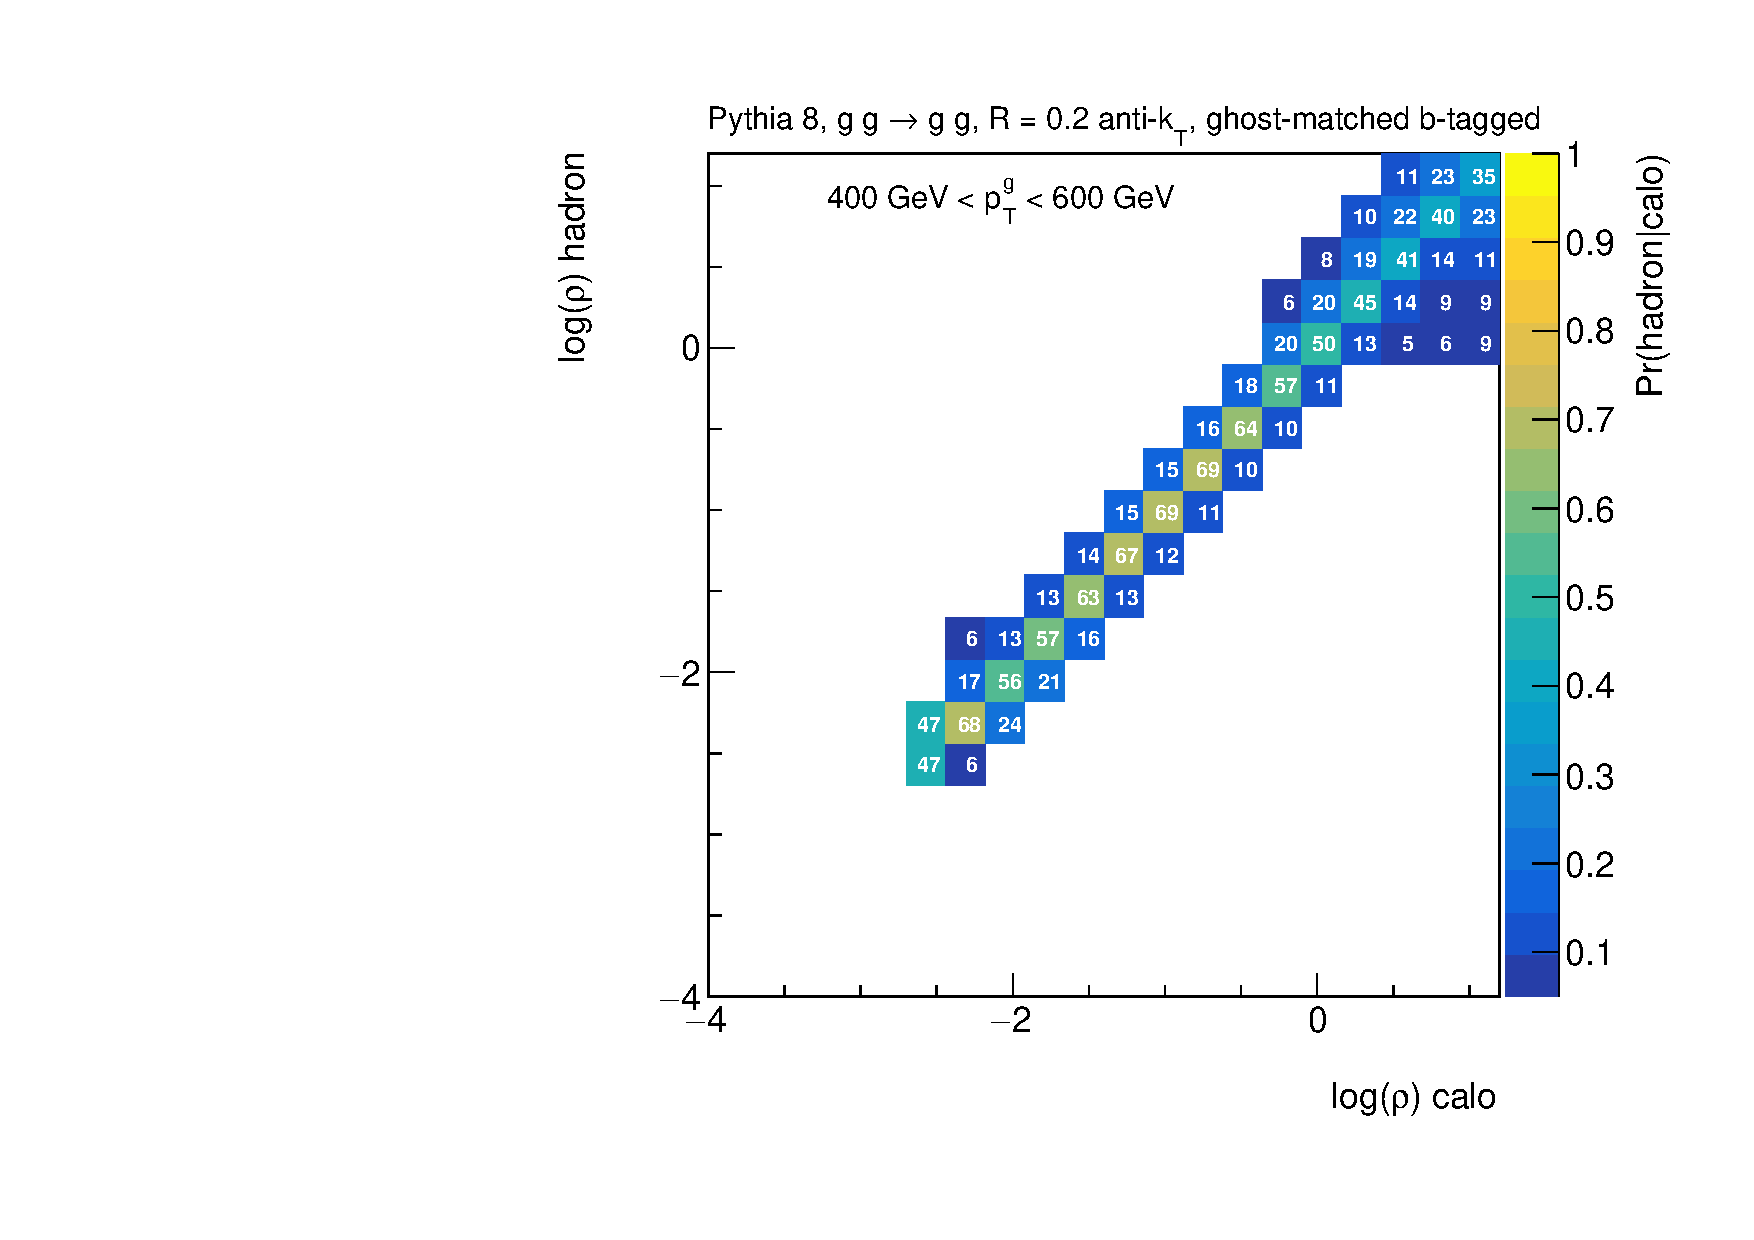
\includegraphics[width=0.45\linewidth]{figures/gbb/truth_level/rho_calo_track_b.pdf}
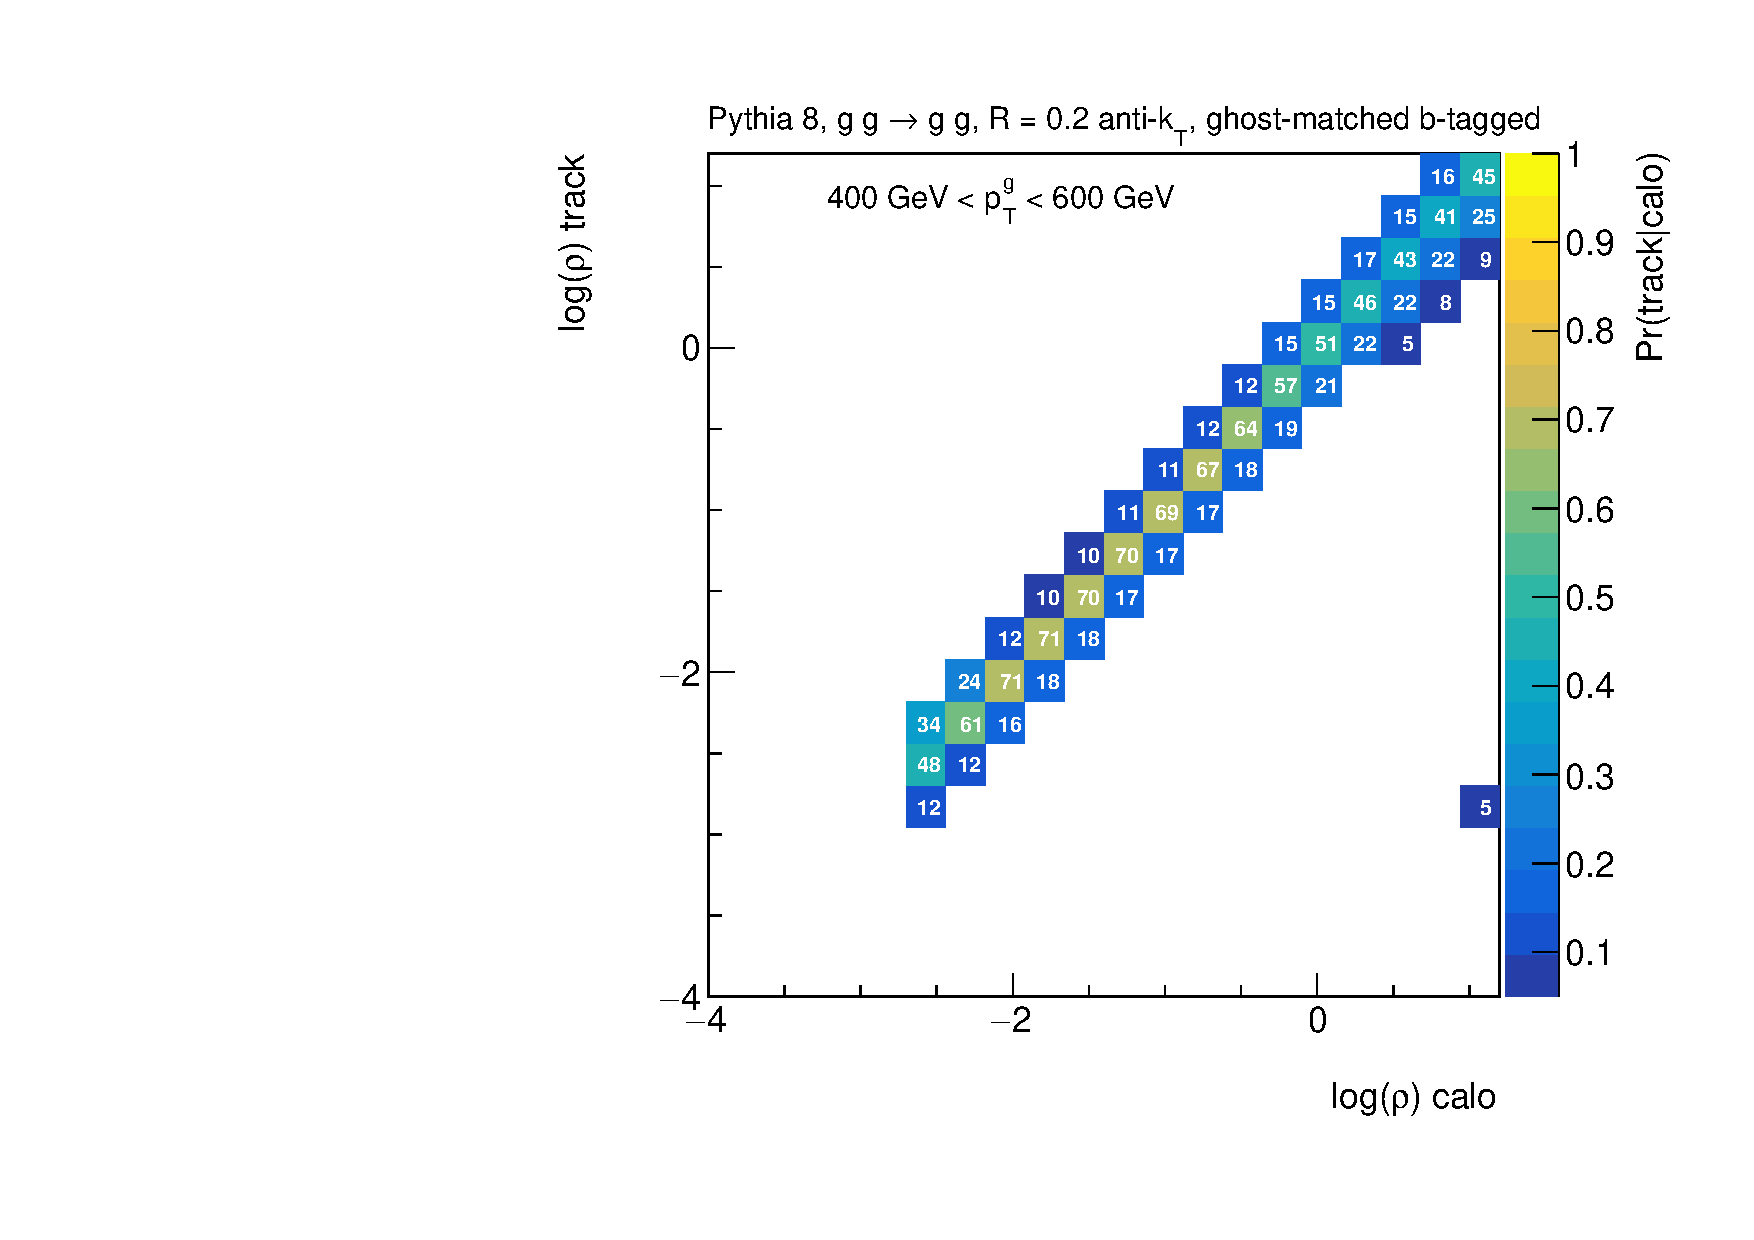
\includegraphics[width=0.45\linewidth]{figures/gbb/truth_level/rho_calo_track.pdf}
\caption{The two-dimensional distribution of two of the variables from Fig.~\ref{fig:gbb-gbbdistributions}, but using different definitions of `b' ($B$-hadrons, $b$-jets, $b$-track-jets).} 
\label{fig:gbb-gbbresponse}
\end{center}
\end{figure}

\begin{figure}[htpb!]
\begin{center}
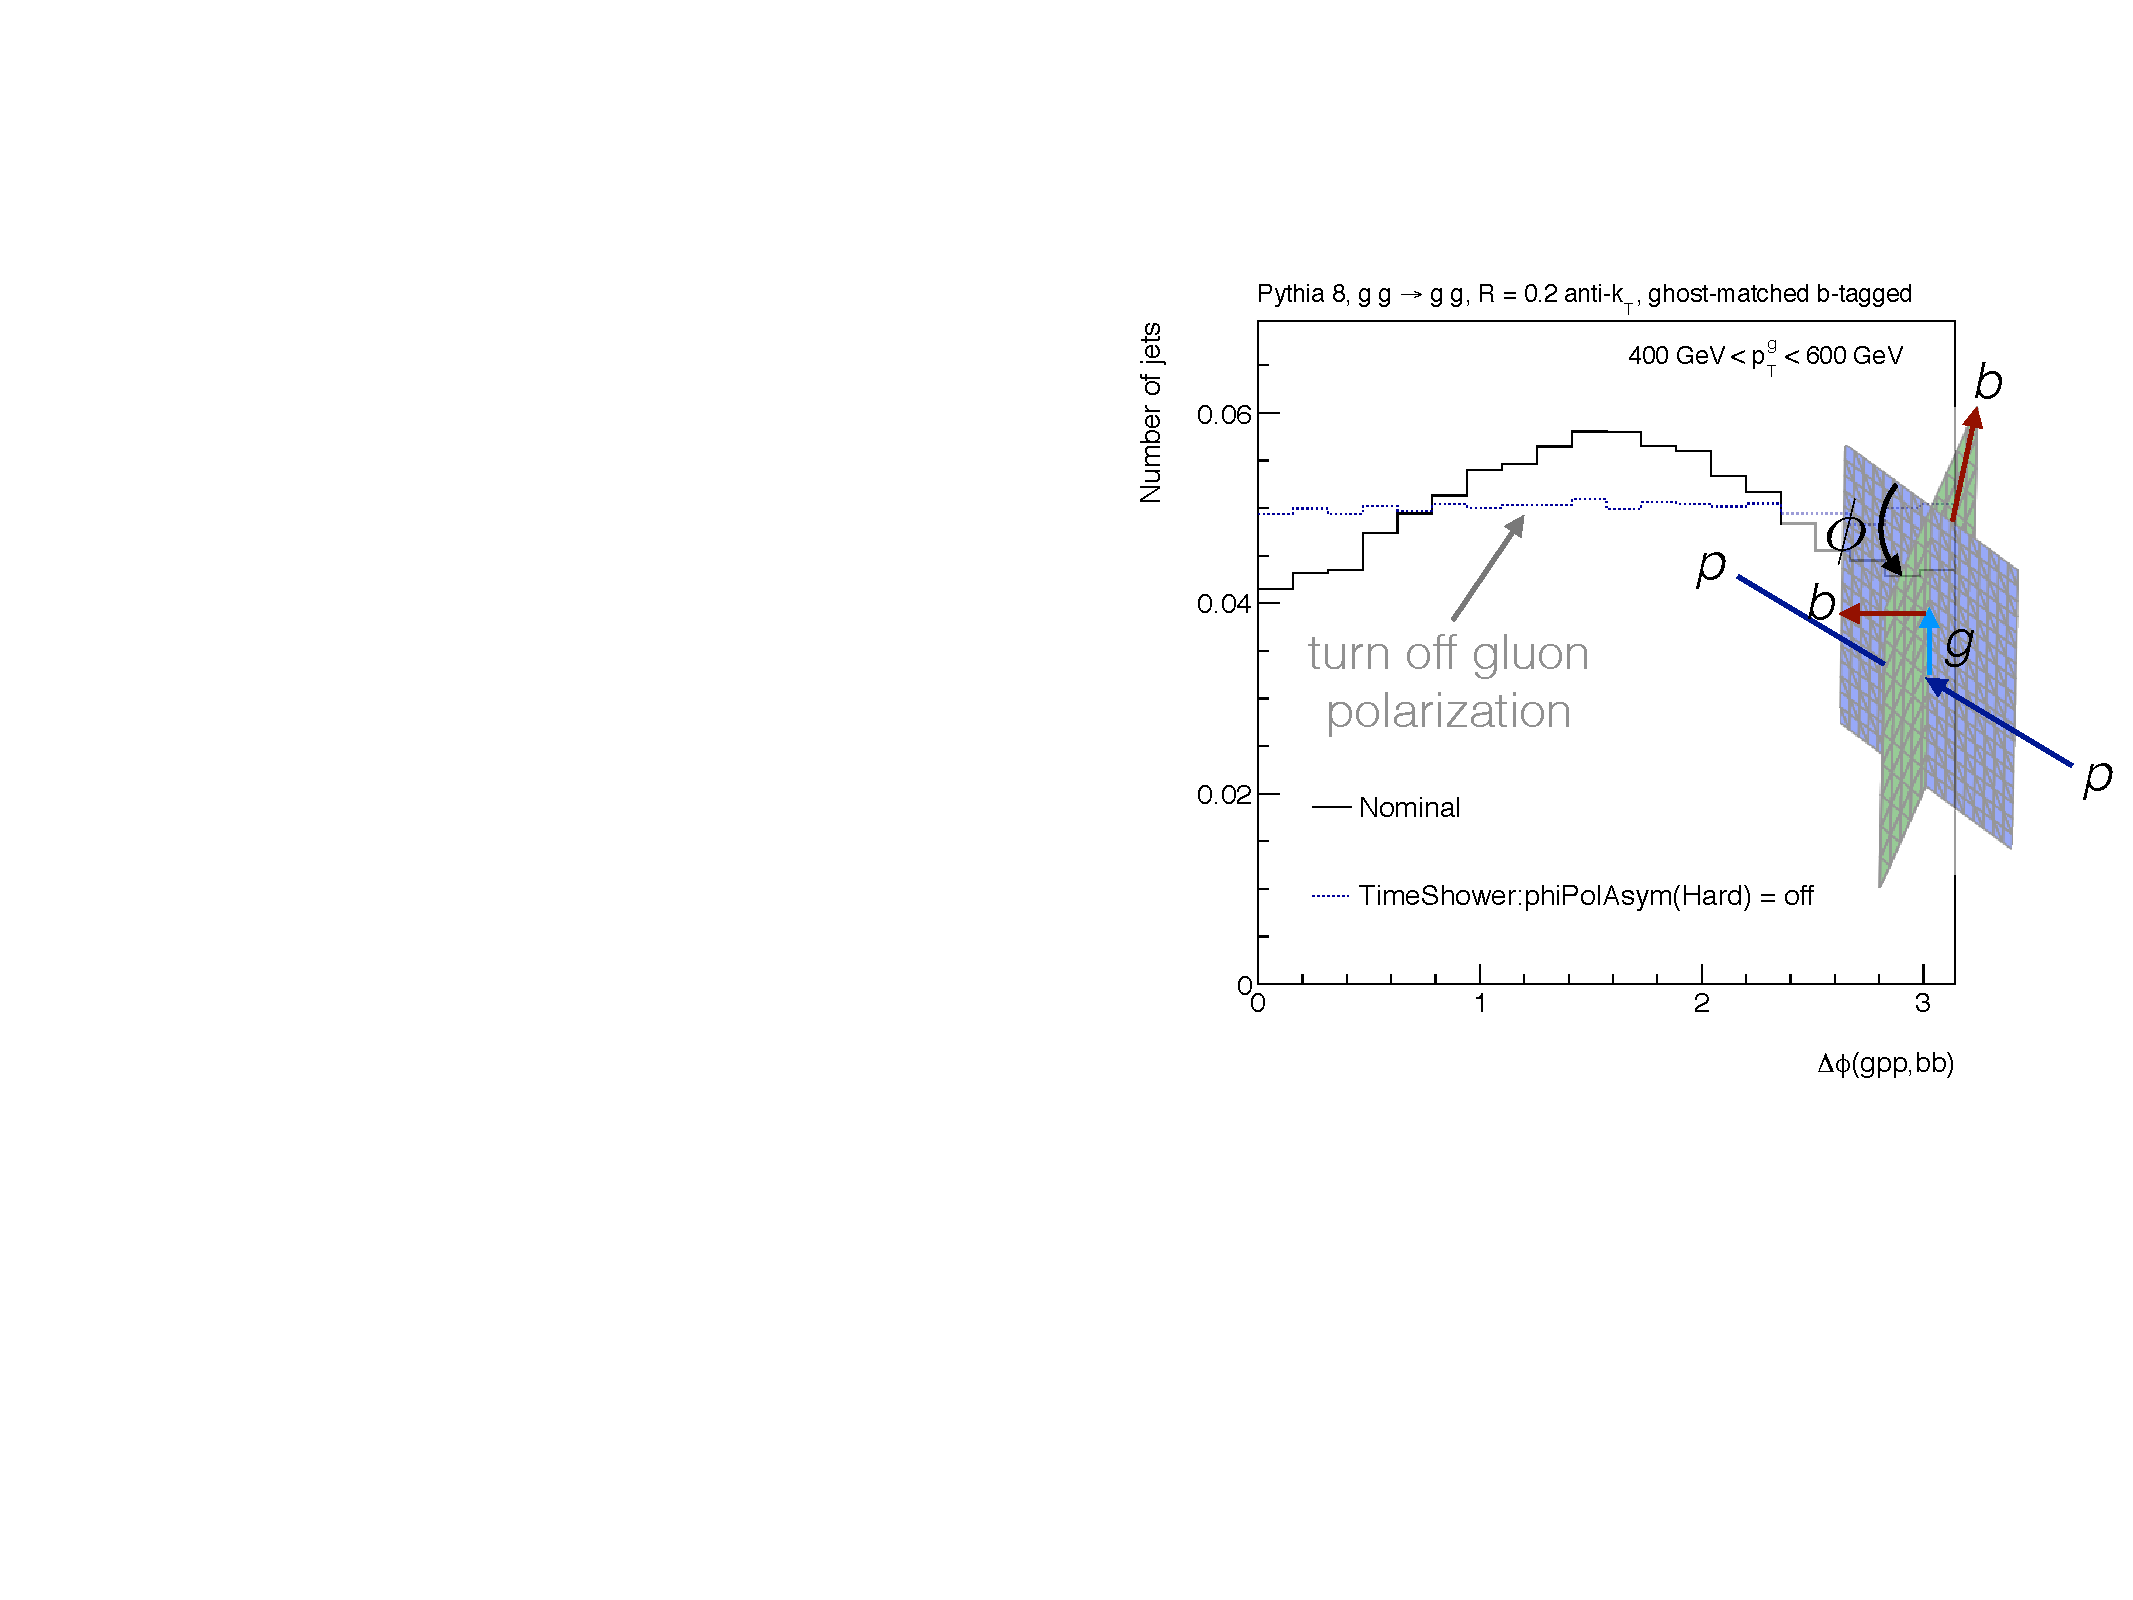
\includegraphics[width=0.45\linewidth]{figures/gbb/truth_level/phi.pdf}
\caption{The angle $\phi$ that the $g\rightarrow b\bar{b}$ plane makes with respect to the $pp\rightarrow g$ plane.  This distribution is sensitive to the gluon polarization.} 
\label{fig:gbb-gbbangle}
\end{center}
\end{figure}

